% !TeX program = xelatex

\section{Deployment}
\label{sec:deployment}

Wie aus den vorhergenden Kapiteln hervorgeht, ist die Anwendung recht groß und besteht aus vielen Komponenten.
Dies macht leider das Deployment der Gesammtanwendung kompliziert.
Daher wurde der Deployment Prozess in mehrere Schritte aufgeteilt, welche in diesem Kapitel beschrieben werden.


\subsection{Deployment der Anwendung}
Die Anwendung bzw. Anwendungen, aus welchen das Projekt zusammengebaut wurde, sind alle um das Docker Ökosystem aufgebaut (siehe \ref{sec:docker}).
Einzelne Komponenten sind mit Docker Files ausgestattet um die entsprechenden Images zu bauen.
Zum starten aller Container wurden zwei unterschiedliche Docker Compose Dateien erstellt, eines für die Entwicklung und eines für die Produktion. Das zweite wurde mit den auch in \ref{cha:setup} vorgestellten Überwachungstools ausgestattet.

Es wurde auch ein Template für die Docker Swarm Orchestrierung erstellt, welches das ganze Projekt in einer stabilen Umgebung laufen lässt und dem Betreiber die Möglichkeit gibt, die Anwendung auf mehreren Servern zu verteilen. 
Hier müssten lediglich die gewünschten Bedienung noch definiert werden.


\subsection{Automatisierung der Deployment Pipeline}
\label{sec:deployment_pipeline}

Da der ganze Prozess des manuellen Deployment sehr aufwendig ist, wurde eine automatisierte Deployment Pipeline erstellt.
Diese läuft über die GitLab CI/CD Funktionen und wird bei jedem Push auf den Master Branch ausgeführt.
Hierfür muss lediglich ein passender Runner auf dem Server installiert sein, welcher die Jobs ausführt. Die entsprechenden Variable müssen in der GitLab CI/CD Konfiguration hinterlegt werden und schon wird der Prozess bei jedem Push ausgeführt.

Der Prozess, abgebildet in Abbildung \ref{fig:deployment_process}, besteht aus folgenden Schritten:
\begin{enumerate}
    \item Baue die Django, Spring, Hugo und React Images
    \item Lade die Images auf den Server
    \item Ersetzte die Container Image Tags durch die neuen Tags der Images, hierfür wird das Template genutzt
    \item Deploye den Stack auf dem Server, Treafik wird als Manager gesetzt
\end{enumerate}


\begin{figure}[h]
    \centering
    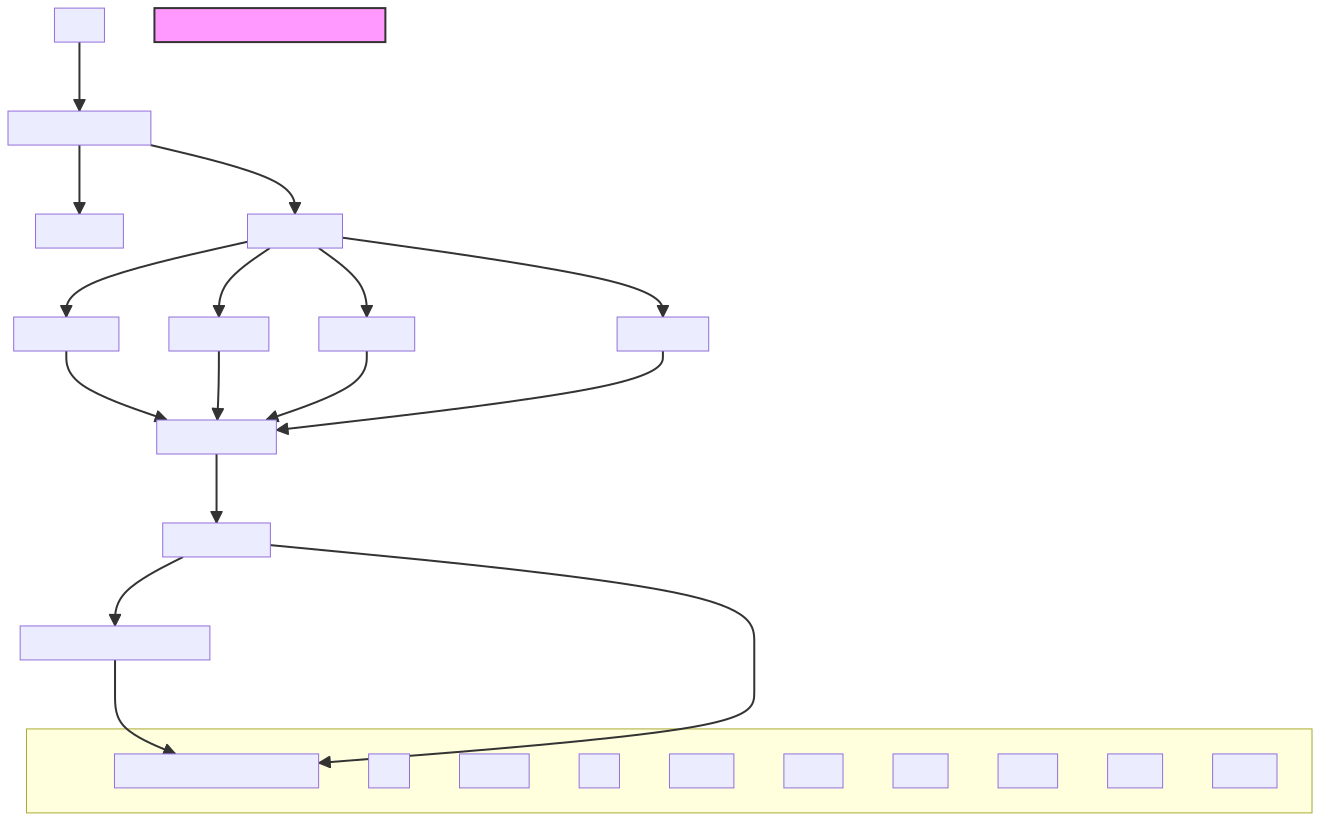
\includegraphics[width=1\textwidth,height=\textheight,keepaspectratio]{includes/figures/docker_deployment.png}
    \caption{Visuelle Darstellung des Deployment Prozesses in GitLab CI/CD und lokaler Umgebung}
    \label{fig:deployment_process}
\end{figure}


Der Prozess ist in der Datei \textit{.gitlab-ci.yml} hinterlegt und kann dort angepasst werden.
Wie in Abbildung \ref{fig:gitlab_ci_pipeline} zu sehen ist, werden die einzelnen Schritte als Jobs definiert und können auch einzeln ausgeführt werden.
Aktuell ist der Deployment Prozess nur für den Master Branch konfiguriert. Hier kann die eigene Vorgehensweise später gewählt werden.
Da aber im aktuellen Prozess nur vom Master abgezweigt wird und dieser immer im Produktivmodus zu laufen hat, gab es keine Notwendigkeit auf eine Git Flow basierte Branching Strategie zu wechseln. 
Dies wäre aber auch möglich, da die GitLab CI/CD Konfiguration auch auf Branches angewendet werden kann.




\begin{figure}[ht]
    \centering
    \begin{minipage}{0.5\textwidth}
        \centering
        \includegraphics[width=\textwidth,height=\textheight,keepaspectratio]{includes/figures/code/code.png}
        \caption{Docker Compose File für den Produktionsprozess}
        \label{fig:code}
    \end{minipage}\hfill
    \begin{minipage}{0.5\textwidth}
        \centering
        \includegraphics[width=\textwidth,height=\textheight,keepaspectratio]{includes/figures/code/gitlab_ci.png}
        \caption{Gitlab CI/CD Pipeline}
        \label{fig:gitlab_ci_pipeline}
    \end{minipage}
\end{figure}
